\chapter{Precipitação e solubilidade}\label{ch:b1:precipitation}

Uma gota de nitrato de prata cai na água da torneira e aparece uma nuvem
branca: cloreto de prata, formado a partir dos poucos miligramas de íons
cloreto contidos em cada litro. A água que se infiltra no calcário leva
embora o carbonato de cálcio e o deposita de novo, uma fração de
milímetro por ano, nas estalactites de uma caverna. Um cálculo renal
também é um precipitado. Cada um desses casos é um equilíbrio entre um
sólido e seus íons em solução, e uma única constante, o \omterm{def:b1:precipitation:solubility-product}{produto de
solubilidade}, diz se o sólido se forma, quanto dele se dissolve e como
sua \omterm{def:b1:precipitation:solubility}{solubilidade} varia quando se altera outro íon ou o pH. Com ela, o
químico pode separar os íons uns dos outros precipitando-os um de cada
vez --- a base do tratamento das águas de mina que encerra este
capítulo.

\begin{recall}
O volume escolar (anos 6 e 12) mediu a \omterm{def:b1:precipitation:solubility}{solubilidade} em gramas por litro
e identificou íons pelos precipitados que eles dão. A constante de
equilíbrio, o \omterm{def:b1:extent-q-and-k:quotient}{quociente de reação} $Q$ e as \omterm{def:b1:extent-q-and-k:activity}{atividades} (1 para um sólido
puro ou para o solvente, $c/c^\circ$ para um soluto) foram estabelecidos
no \cref{ch:b1:extent-q-and-k}: uma reação avança enquanto $Q < K$. O
método da \omterm{def:b1:predominant-reaction:predominant-reaction}{reação predominante} e a escala de $\mathrm{p}K_a$ vêm do
\cref{ch:b1:predominant-reaction}; $c^\circ = \qty{1}{mol/L}$ não é
escrito nos quocientes.
\end{recall}

\begin{omfigure}
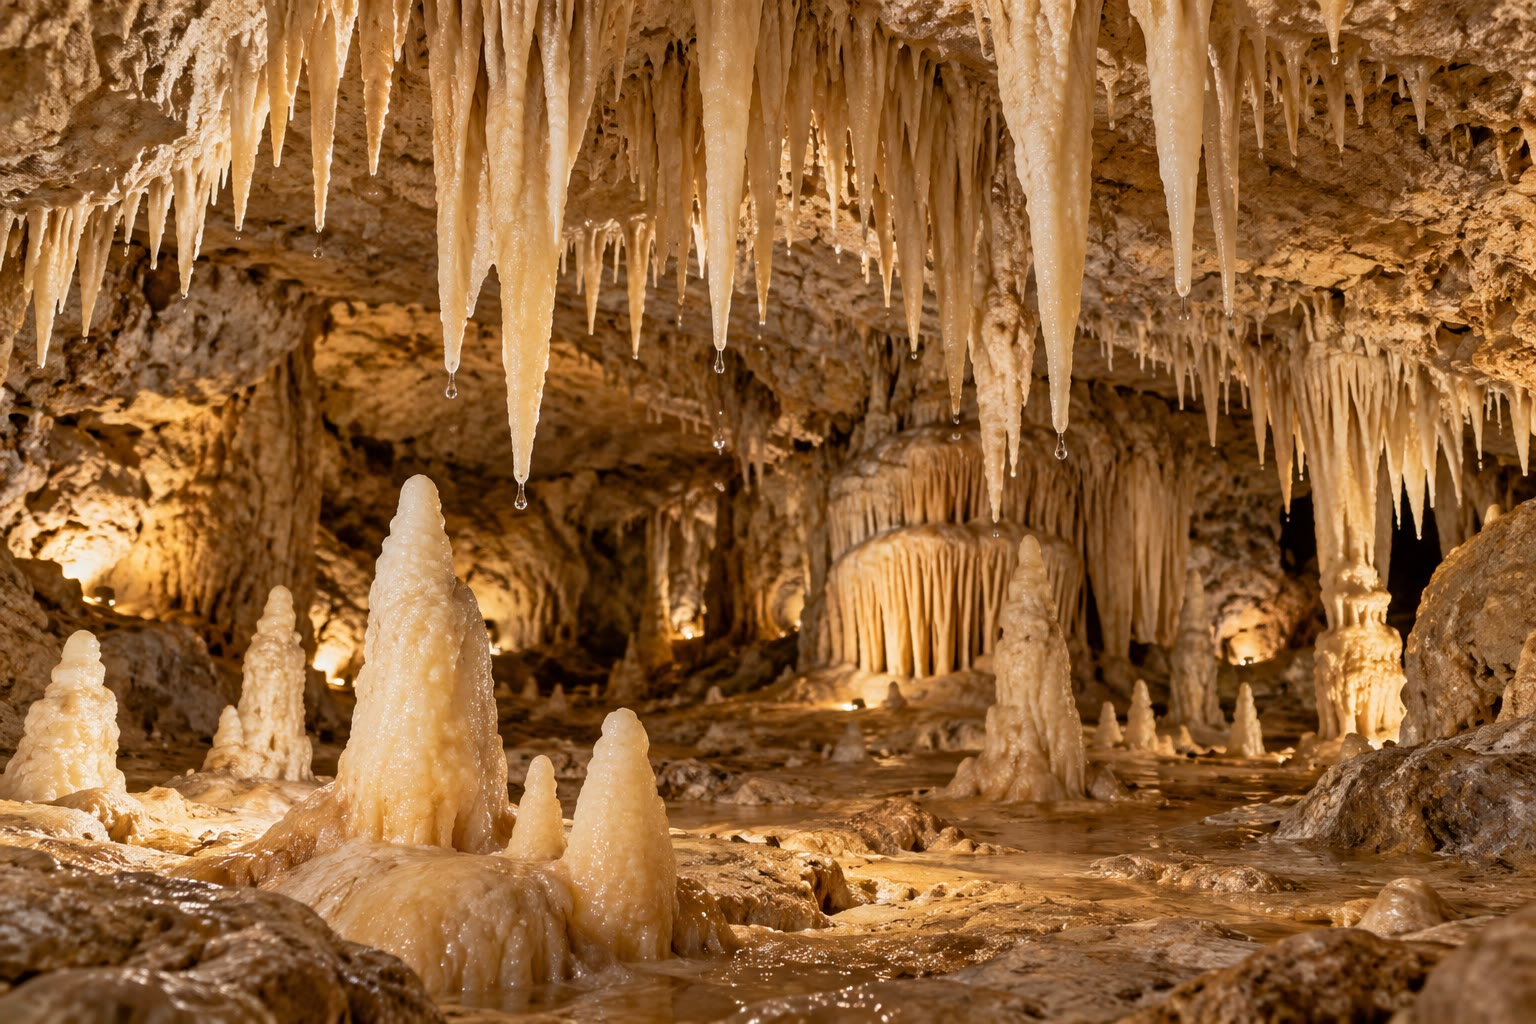
\includegraphics[width=0.62\linewidth]{images/book2/ai/b1-11-cave.jpg}

{\small Estalactites e estalagmites em uma caverna calcária. A água rica
em dióxido de carbono dissolve o carbonato de cálcio no solo acima; na
caverna, ela perde parte de seu dióxido de carbono e o carbonato
precipita de novo (\cref{exo:b1:precipitation:10}).}
\end{omfigure}

\section{O produto de solubilidade}\label{sec:b1:precipitation:product}

Um \omterm{def:b1:crystals-metals:crystal}{cristal} de cloreto de prata colocado na água cede íons à solução, e a
solução devolve alguns ao \omterm{def:b1:crystals-metals:crystal}{cristal}. Quando as duas velocidades se
igualam, a solução está \emph{saturada}: sua composição não varia mais,
embora os íons continuem passando nos dois sentidos (figura abaixo).

\begin{definition}[Produto de solubilidade]\label{def:b1:precipitation:solubility-product}
O \emph{produto de solubilidade}\index{produto de solubilidade} $K_s$ de um
sólido iônico $\mathrm{M}_a\mathrm{X}_b$ é a constante de equilíbrio de
sua dissolução em seus íons,
\[
  \mathrm{M}_a\mathrm{X}_b\mathrm{(s)} \rightleftharpoons a\,\mathrm{M}^{m+}
  + b\,\mathrm{X}^{x-}, \qquad
  K_s = [\mathrm{M}^{m+}]_{\mathrm{eq}}^{\,a}\,[\mathrm{X}^{x-}]_{\mathrm{eq}}^{\,b},
  \qquad \mathrm{p}K_s = -\log K_s ,
\]
sendo 1 a \omterm{def:b1:extent-q-and-k:activity}{atividade} do sólido. Como toda constante de equilíbrio, ele só
depende da temperatura.
\end{definition}

Para o cloreto de prata, \ce{AgCl(s) <=> Ag+ + Cl-} e $K_s =
[\ce{Ag+}][\ce{Cl-}] = 10^{-9.75}$; para o fluoreto de cálcio, \ce{CaF2(s) <=>
Ca^2+ + 2F-} e $K_s = [\ce{Ca^2+}][\ce{F-}]^2 = 10^{-9.84}$; para o
hidróxido de ferro(III), $K_s = [\ce{Fe^3+}][\ce{OH-}]^3 = 10^{-38.55}$.
A tabela abaixo reúne os valores usados neste volume.
Eles são calculados, como os $\mathrm{p}K_a$ do
\cref{ch:b1:predominant-reaction}, a partir das energias de Gibbs padrão
de formação tabeladas: $\mathrm{p}K_s = \Delta_r G^\circ/(RT\ln 10)$,
relação deduzida no volume do 2.º~ano.

\begin{omfigure}
\begin{tikzpicture}[font=\small, >={Stealth}]
  % the crystal: alternating Ag+ (small, grey) and Cl- (large, green)
  \foreach \i in {0,1,2,3,4,5}
    \foreach \j in {0,1,2} {
      \pgfmathtruncatemacro{\pp}{mod(\i+\j,2)}
      \ifnum\pp=0
        \shade[ball color=green!55!black!60] (\i*0.62,\j*0.62) circle (0.29);
      \else
        \shade[ball color=gray!35] (\i*0.62,\j*0.62) circle (0.17);
      \fi }
  \draw[thick, gray] (-0.45,-0.45) rectangle (3.55,1.75);
  \node[below] at (1.55,-0.45) {\ce{AgCl(s)}};
  % ions in solution
  \shade[ball color=gray!35] (1.2,3.0) circle (0.17);
  \node[right] at (1.4,3.0) {\ce{Ag+}};
  \shade[ball color=green!55!black!60] (2.6,2.7) circle (0.29);
  \node[right] at (2.9,2.7) {\ce{Cl-}};
  \shade[ball color=gray!35] (4.4,1.4) circle (0.17);
  \shade[ball color=green!55!black!60] (5.1,2.6) circle (0.29);
  \shade[ball color=gray!35] (-1.0,2.4) circle (0.17);
  \shade[ball color=green!55!black!60] (-0.6,3.3) circle (0.29);
  % arrows: dissolution and precipitation
  \draw[->, thick, omDef] (1.24,1.6) to[bend left=20] node[left, pos=0.6] {dissolução} (1.15,2.78);
  \draw[->, thick, omProp] (2.55,2.38) to[bend left=20] node[right, pos=0.45] {precipitação} (2.45,1.55);
  % the water line
  \draw[blue!50, thick] (-1.6,3.8) -- (5.9,3.8);
  \node[blue!60!black, anchor=east] at (5.9,4.05) {solução saturada};
\end{tikzpicture}

{\small Um \omterm{def:b1:crystals-metals:crystal}{cristal} de cloreto de prata em sua solução saturada. Íons
deixam a superfície (dissolução) e outros são capturados (precipitação)
na mesma velocidade, de modo que $[\ce{Ag+}][\ce{Cl-}]$ permanece igual a
$K_s$. Os íons prata são desenhados menores que os íons cloreto, como de
fato são.}
\end{omfigure}

\begin{omfigure}
\begin{tabular}{lc@{\qquad}lc}
\hline
sólido & $\mathrm{p}K_s$ & sólido & $\mathrm{p}K_s$ \\
\hline
\ce{AgCl} & 9.75 & \ce{Ca(OH)2} & 5.33 \\
\ce{AgBr} & 12.27 & \ce{Mg(OH)2} & 11.25 \\
\ce{AgI} & 16.07 & \ce{Fe(OH)2} & 16.31 \\
\ce{Ag2CrO4} & 11.95 & \ce{Zn(OH)2} & 16.38 \\
\ce{BaSO4} & 9.97 & \ce{Fe(OH)3} & 38.55 \\
\ce{CaCO3} (calcita) & 8.30 & \ce{Al(OH)3} (gibbsita) & 34.75 \\
\ce{CaF2} & 9.84 & & \\
\hline
\end{tabular}

\smallskip
{\small \omterm{def:b1:precipitation:solubility-product}{Produtos de solubilidade} a \qty{25}{\celsius}, calculados a
partir das energias de Gibbs padrão de formação dos sólidos e dos íons
aquosos. Constantes de formação usadas neste capítulo
(\cref{sec:b1:precipitation:amphoteric}):
$\log\beta_4 = 14.45$ para \ce{Zn(OH)4^2-}, 33.52 para \ce{Al(OH)4-}, e
$\log\beta_1 = 11.82$ para \ce{FeOH^2+}.}
% ledger: dfg:AgCl_cr, dfg:AgBr_cr, dfg:AgI_cr, dfg:Ag2CrO4_cr, dfg:Ag+_ao, dfg:Cl-_ao, dfg:Br-_ao, dfg:I-_ao, dfg:CrO42-_ao (computed in figdata/bachelor-1/aqueous-constants.py)
% ledger: dfg:BaSO4_cr, dfg:Ba2+_ao, dfg:SO42-_ao, dfg:CaCO3_cr, dfg:CO32-_ao, dfg:CaF2_cr, dfg:Ca2+_ao, dfg:F-_ao (computed, same script)
% ledger: dfg:Ca_OH2_cr, dfg:Mg_OH2_cr, dfg:Mg2+_ao, dfg:Fe_OH2_cr, dfg:Fe2+_ao, dfg:Zn_OH2_cr, dfg:Zn2+_ao, dfg:Fe_OH3_cr, dfg:Fe3+_ao, dfg:Al2O3.3H2O_cr, dfg:Al3+_ao, dfg:OH-_ao (computed, same script)
% ledger: dfg:Zn_OH42-_ao, dfg:Al_OH4-_ao, dfg:FeOH2+_ao (formation constants, same script)
\end{omfigure}

\begin{proposition}[Condição de precipitação]\label{prop:b1:precipitation:precipitation-condition}
Considere uma solução que contém os íons de um sólido
$\mathrm{M}_a\mathrm{X}_b$, com \omterm{def:b1:extent-q-and-k:quotient}{quociente de reação}
$Q_s = [\mathrm{M}^{m+}]^a[\mathrm{X}^{x-}]^b$ para a dissolução.
\begin{itemize}
  \item Se $Q_s < K_s$, o sólido não pode estar presente no equilíbrio: a
        solução não está saturada e todo sólido adicionado se dissolve,
        completamente se não houver demais.
  \item Se $Q_s > K_s$, o sólido precipita até que $Q_s = K_s$.
  \item O sólido e a solução só coexistem em equilíbrio quando
        $Q_s = K_s$.
\end{itemize}
\end{proposition}

\begin{proof}
Pelo \cref{ch:b1:extent-q-and-k}, a dissolução avança enquanto
$Q_s < K_s$ e recua (precipitação) enquanto $Q_s > K_s$. Enquanto a
dissolução avança, $Q_s$ aumenta. Se o sólido se esgota antes de $Q_s$
atingir $K_s$, a evolução para sem que reste sólido: uma reação que
envolve uma \omterm{def:b1:extent-q-and-k:system}{fase} condensada pura pode parar antes do equilíbrio, porque
a quantidade dessa \omterm{def:b1:extent-q-and-k:system}{fase} não pode ficar negativa. Se $Q_s > K_s$, a
precipitação diminui as duas concentrações iônicas e $Q_s$ diminui até
igualar $K_s$, o que sempre é possível, já que os íons estão presentes.
\end{proof}

O último ponto é o que distingue um sólido de uma espécie dissolvida.
Uma espécie ácido--base está presente em qualquer pH, por menor que
seja sua concentração; um sólido está presente ou ausente. É por isso
que seu diagrama será um diagrama de \emph{existência}, e não de
predominância (\cref{sec:b1:precipitation:domains}).

\begin{example}[Misturar duas soluções]\label{ex:b1:precipitation:mixing}
Misturam-se \qty{10.0}{mL} de nitrato de prata a \qty{2.0e-4}{mol/L} com
\qty{10.0}{mL} de cloreto de sódio a \qty{2.0e-4}{mol/L}. Logo após a
mistura, antes de qualquer reação, $[\ce{Ag+}] = [\ce{Cl-}] = \qty{1.0e-4}{mol/L}$
e $Q_s = 10^{-8.0} > K_s = 10^{-9.75}$: o cloreto de prata precipita.
Com as duas soluções a \qty{2.0e-6}{mol/L}, $Q_s = 10^{-12.0} < K_s$ e a
mistura fica límpida. O nitrato de prata é um teste sensível para os
íons cloreto, mas não infinitamente sensível.
\end{example}

\begin{inthelab}[O teste do cloreto]
No laboratório de ensino, algumas gotas de solução de nitrato de prata
são adicionadas à amostra, previamente acidificada com ácido nítrico
diluído. O ácido transforma os íons carbonato e hidróxido em dióxido de
carbono e água, que de outro modo também precipitariam com os íons
prata. Um precipitado branco que escurece à luz é cloreto de prata; o
brometo dá um precipitado creme e o iodeto, um amarelo
(fotografia abaixo).
O nitrato de prata mancha a pele de preto: usam-se luvas e óculos.
\end{inthelab}

\begin{omfigure}
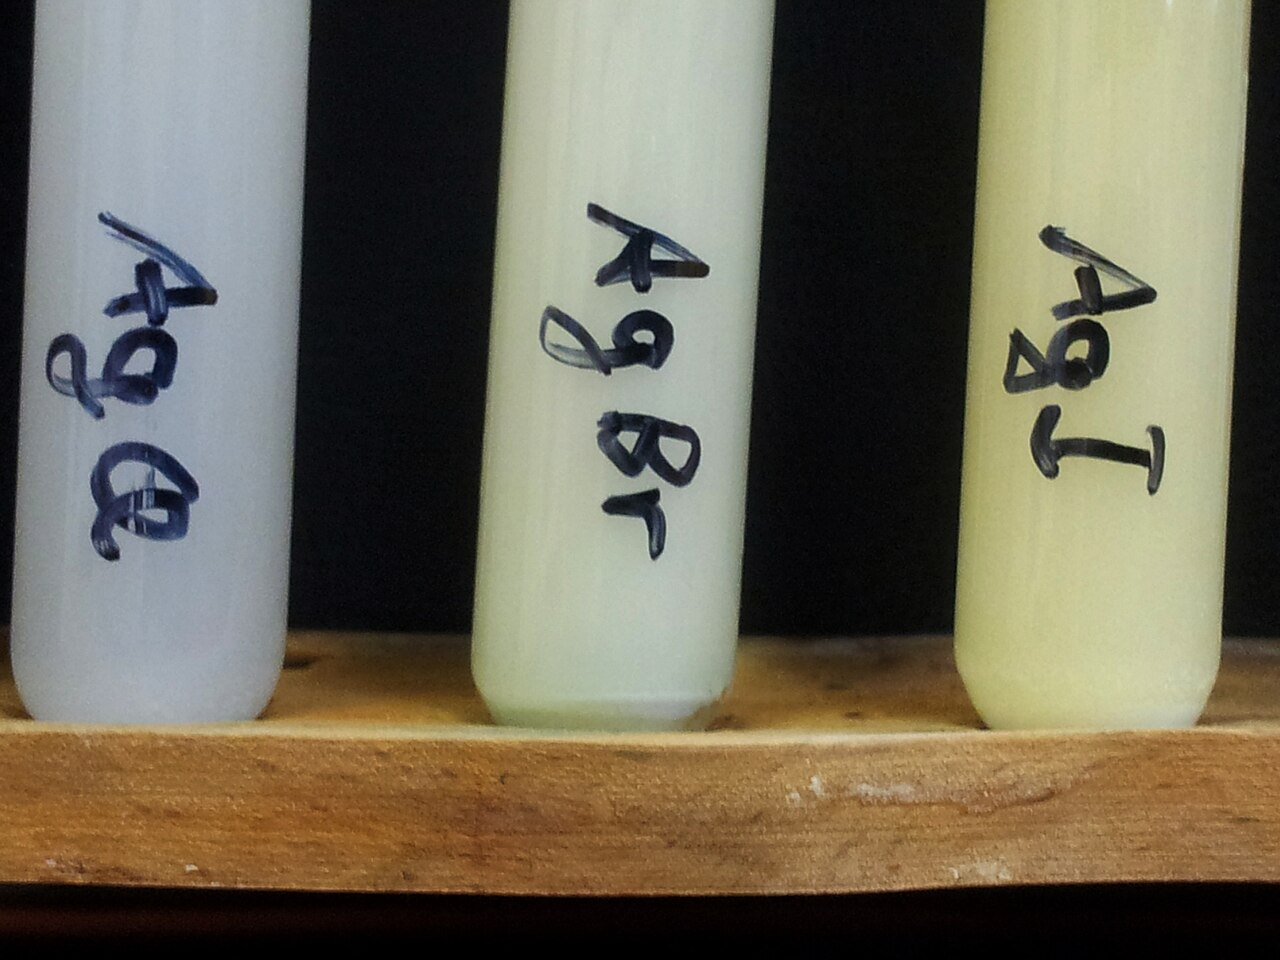
\includegraphics[width=0.6\linewidth]{images/book2/silver-halides.jpg}

{\small Precipitados de cloreto de prata (branco), brometo de prata
(creme) e iodeto de prata (amarelo-claro). Fotografia de Rrausch1974,
CC BY-SA 3.0, Wikimedia Commons.}
\end{omfigure}

\section{Solubilidade}

\begin{definition}[Solubilidade]\label{def:b1:precipitation:solubility}
A \emph{solubilidade}\index{solubilidade} $s$ de um sólido em uma dada
solução é a quantidade de sólido que se dissolve em um litro dessa
solução até a saturação (em \unit{mol/L}); multiplicada pela massa molar,
é a solubilidade mássica, em \unit{g/L}. Ela depende da temperatura e da
composição da solução.
\end{definition}

\begin{proposition}[Solubilidade a partir do produto de solubilidade]\label{prop:b1:precipitation:s-of-ks}
Em água pura, se os íons não participam de nenhuma outra reação,
\[
  \mathrm{MX}:\ s = \sqrt{K_s}, \qquad
  \mathrm{MX_2}\ \text{ou}\ \mathrm{M_2X}:\ s = \left(\frac{K_s}{4}\right)^{1/3},
  \qquad
  \mathrm{M}_a\mathrm{X}_b:\ s = \left(\frac{K_s}{a^a b^b}\right)^{1/(a+b)} .
\]
\end{proposition}

\begin{proof}
Quando $s$ mol de sólido se dissolvem por litro, $[\mathrm{M}^{m+}] = as$ e
$[\mathrm{X}^{x-}] = bs$, logo, na saturação, $K_s = (as)^a(bs)^b =
a^a b^b s^{a+b}$. Para MX, $a = b = 1$; para \ce{MX2}, $1^1 2^2 = 4$, e o
mesmo para \ce{M2X}.
\end{proof}

\begin{example}[Cloreto de prata e cromato de prata]\label{ex:b1:precipitation:agcl-ag2cro4}
Cloreto de prata: $s = 10^{-9.75/2} = \qty{1.3e-5}{mol/L}$, ou seja,
\qty{1.9}{mg/L} com $M = \qty{143.4}{g/mol}$. Cromato de prata \ce{Ag2CrO4}
($\mathrm{p}K_s = 11.95$): $s = (10^{-11.95}/4)^{1/3} =
\qty{6.6e-5}{mol/L}$. O cromato tem o menor $K_s$ e, no entanto, é cinco
vezes mais solúvel. Os \omterm{def:b1:precipitation:solubility-product}{produtos de solubilidade} só podem ser comparados
diretamente entre sólidos de mesmo tipo de fórmula.
\end{example}

\begin{remark}
As fórmulas supõem que os íons estão livres. Em água pura, o íon cromato
é uma \omterm{def:b1:predominant-reaction:strong-acid}{base fraca} e o íon prata não é complexado por nada, de modo que o
resultado para o cromato de prata é quase correto; para um carbonato,
um sulfeto ou um hidróxido, as propriedades básicas do ânion importam e
é preciso a seção seguinte. Em força iônica elevada, as \omterm{def:b1:extent-q-and-k:activity}{atividades}
também se afastam das concentrações, correção deixada para o volume do
2.º~ano.
\end{remark}

\section{Efeitos do íon comum e do pH}

\begin{definition}[Efeito do íon comum]\label{def:b1:precipitation:common-ion}
O \emph{efeito do íon comum}\index{efeito do ion comum@efeito do íon comum} é a diminuição
da \omterm{def:b1:precipitation:solubility}{solubilidade} de um sólido em uma solução que já contém um de seus
íons.
\end{definition}

\begin{proposition}[Solubilidade com um íon comum]\label{prop:b1:precipitation:common-ion}
Seja MX que se dissolve em uma solução em que já se tem
$[\mathrm{X}^-] = c$, com $c \gg \sqrt{K_s}$. Então $s \approx K_s/c$,
muito menor que em água pura. Para \ce{MX2} em uma solução que contém
\ce{M^2+} a $c$,
$s \approx \frac12\sqrt{K_s/c}$.
\end{proposition}

\begin{proof}
Na saturação, $[\mathrm{M}^+] = s$ e $[\mathrm{X}^-] = c + s$, logo
$s(c + s) = K_s$. Se $s \ll c$, $s = K_s/c$; a suposição se verifica, pois
$K_s/c \ll c$ quando $c^2 \gg K_s$. Para \ce{MX2}, $[\ce{X-}] = 2s$ e
$[\mathrm{M}^{2+}] = c + s \approx c$, logo $c\,(2s)^2 = K_s$.
\end{proof}

Cloreto de prata em cloreto de sódio a \qty{0.10}{mol/L}: $s = 10^{-9.75}/0.10
= \qty{1.8e-9}{mol/L}$, sete mil vezes menos que em água. É por isso que
um precipitado é lavado com uma solução diluída de um íon comum, e não
com água pura: ele perde menos de si mesmo.

Quando o ânion do sólido é uma base, o ácido o retira do equilíbrio de
dissolução e a \omterm{def:b1:precipitation:solubility}{solubilidade} aumenta. Para o carbonato de cálcio em meio
ácido,
\[
  \ce{CaCO3(s) + H3O+ <=> Ca^2+ + HCO3- + H2O}, \qquad
  K = \frac{K_s}{K_{a2}} = 10^{-8.30 + 10.33} = 10^{2.03} ,
\]
uma reação favorecida: o vinagre ou o ácido clorídrico dissolvem o
calcário, e o dióxido de carbono formado pela reação seguinte do
\ce{HCO3-} produz a efervescência conhecida.
% ledger: dfg:HCO3-_ao (pKa2 of carbonic acid, ch. 10)

\begin{proposition}[Solubilidade de um hidróxido em função do pH]\label{prop:b1:precipitation:hydroxide-ph}
Em uma solução tamponada em um dado pH, a concentração de \ce{M^{n+}} em
equilíbrio com o hidróxido \ce{M(OH)_n} obedece a
\[
  \log[\mathrm{M}^{n+}] = -\mathrm{p}K_s + n\,(\mathrm{p}K_e - \mathrm{pH}) ,
\]
uma reta de inclinação $-n$ em função do pH. Se o íon não forma nenhum
complexo, essa é a \omterm{def:b1:precipitation:solubility}{solubilidade} do hidróxido.
\end{proposition}

\begin{proof}
$K_s = [\mathrm{M}^{n+}][\ce{OH-}]^n$ e $[\ce{OH-}] = K_e/[\ce{H3O+}]$,
logo $\log[\mathrm{M}^{n+}] = \log K_s - n\log[\ce{OH-}] = -\mathrm{p}K_s -
n(\mathrm{pH} - \mathrm{p}K_e)$.
\end{proof}

Cada unidade de pH divide a \omterm{def:b1:precipitation:solubility}{solubilidade} do hidróxido de ferro(III) por
mil e a do hidróxido de zinco por cem. Os hidróxidos são precipitados,
e dissolvidos de novo, variando-se o pH.

\begin{example}[Dissolver o carbonato de cálcio com dióxido de carbono]\label{ex:b1:precipitation:cave}
A água que contém dióxido de carbono dissolvido dissolve a calcita:
\[
  \ce{CaCO3(s) + CO2(aq) + H2O <=> Ca^2+ + 2HCO3-}, \qquad
  K = \frac{K_s K_{a1}}{K_{a2}} = 10^{-8.30 - 6.37 + 10.33} = 10^{-4.34} ,
\]
sendo a constante obtida somando a dissolução do carbonato, a primeira
acidez do dióxido de carbono e o inverso da segunda. Quanto mais dióxido
de carbono, mais carbonato de cálcio se dissolve. O ar do solo costuma
ser muito mais rico em dióxido de carbono que o ar de uma caverna; a
água que atravessou o solo e chega ao teto da caverna perde dióxido de
carbono, e a calcita se deposita (\cref{exo:b1:precipitation:10}).
\end{example}

\section{Domínios de existência e precipitação seletiva}\label{sec:b1:precipitation:domains}

\begin{definition}[Domínio de existência]\label{def:b1:precipitation:existence-domain}
Para um sólido e uma dada concentração total $c$ de um de seus íons, o
\emph{domínio de existência}\index{dominio de existencia@domínio de existência} do sólido é o
intervalo da variável (pX, pM ou pH) no qual o sólido está presente no
equilíbrio. Sua fronteira é o valor em que aparece o primeiro grão de
sólido, quando $Q_s = K_s$ com o íon ainda na concentração $c$.
\end{definition}

\begin{method}[Traçar um diagrama de existência]\label{met:b1:precipitation:existence-domain}
\begin{enumerate}
  \item Fixe a concentração total $c$ do íon que não está no eixo (por
        exemplo, $[\ce{Ag+}]_{\mathrm{tot}} = c$ em um eixo de pCl).
  \item Escreva $K_s$ no início da precipitação, com esse íon ainda em
        $c$, e resolva em relação à variável do eixo.
  \item O sólido existe do lado em que o outro íon está concentrado: pCl
        pequeno (muito cloreto), pAg pequeno ou pH alto, para um
        hidróxido.
  \item Não marque um domínio para o próprio íon: ele está presente em
        toda parte, em $c$ fora do domínio do sólido e abaixo de $c$
        dentro dele.
\end{enumerate}
\end{method}

Para o cloreto de prata com $c = [\ce{Ag+}]_{\mathrm{tot}} = 10^{-2}$:
a precipitação começa quando $[\ce{Cl-}] = K_s/c = 10^{-7.75}$, de modo
que o sólido existe para $\mathrm{pCl} < 7.75$. Para o iodeto de prata,
a fronteira fica em $\mathrm{pI} = 16.07 - 2 = 14.07$, como mostra a
figura abaixo.

\begin{omfigure}
\begin{tikzpicture}[font=\small, >={Stealth}, x=0.62cm]
  \fill[omDef!18] (0,0.12) rectangle (7.75,0.6);
  \draw[->, thick] (0,0) -- (17.2,0) node[right] {pCl ou pI};
  \foreach \x in {0,2,4,6,8,10,12,14,16}
    \draw (\x,0.08) -- (\x,-0.08) node[below] {\x};
  \draw[omDef, thick] (7.75,-0.5) -- (7.75,0.9);
  \node[omDef] at (3.9,0.36) {\ce{AgCl(s)} existe};
  \node[omDef, above] at (7.75,0.9) {7.75};
  \node[anchor=west] at (8.0,0.36) {sem sólido: \ce{Ag+} a $10^{-2}$ mol/L};
  % AgI below
  \begin{scope}[yshift=-1.9cm]
  \fill[omProp!20] (0,0.12) rectangle (14.07,0.6);
  \draw[->, thick] (0,0) -- (17.2,0);
  \foreach \x in {0,2,4,6,8,10,12,14,16}
    \draw (\x,0.08) -- (\x,-0.08) node[below] {\x};
  \draw[omProp, thick] (14.07,-0.5) -- (14.07,0.9);
  \node[omProp] at (7.0,0.36) {\ce{AgI(s)} existe};
  \node[omProp, above] at (14.07,0.9) {14.07};
  \end{scope}
\end{tikzpicture}

{\small \omterm{def:b1:precipitation:existence-domain}{Domínios de existência} do cloreto de prata (em um eixo de pCl,
em cima) e do iodeto de prata (em um eixo de pI, embaixo) para uma
concentração total de prata de \qty{1.0e-2}{mol/L}. O iodeto precipita a
prata em concentrações um milhão de vezes menores que o cloreto.}
\end{omfigure}

\begin{method}[Precipitação seletiva]\label{met:b1:precipitation:selective}
Para separar dois íons que precipitam com o mesmo reagente:
\begin{enumerate}
  \item calcule, para cada íon em sua concentração, a concentração de
        reagente (ou o pH) em que seu sólido começa a se formar; o menor
        valor precipita primeiro;
  \item calcule a concentração do primeiro íon que resta em solução
        quando o segundo começa a precipitar;
  \item a separação é aceitável se essa concentração for uma fração
        suficientemente pequena da inicial --- tipicamente \qty{0.1}{\percent}
        --- e o reagente é então interrompido entre os dois limiares.
\end{enumerate}
\end{method}

\begin{example}[Iodeto e cloreto]\label{ex:b1:precipitation:i-cl}
Uma solução contém íons iodeto e cloreto, ambos a
\qty{1.0e-2}{mol/L}; adiciona-se nitrato de prata gota a gota, sem
diluição. O iodeto de prata começa a se formar em $[\ce{Ag+}] = 10^{-16.07 + 2} =
10^{-14.07}$, o cloreto de prata em $10^{-9.75 + 2} = 10^{-7.75}$: o
iodeto precipita primeiro. Quando o cloreto de prata aparece,
$[\ce{I-}] = 10^{-16.07}/10^{-7.75} = 10^{-8.32} = \qty{4.8e-9}{mol/L}$,
uma fração $5 \times 10^{-7}$ do iodeto: a separação é completa.
\end{example}

Os hidróxidos são separados da mesma maneira, com o pH como variável. O
gráfico abaixo mostra, para seis íons a \qty{0.010}{mol/L}, o pH em que
o hidróxido aparece e o pH em que \qty{99.9}{\percent} do íon
precipitou. O ferro(III) e o alumínio são removidos em água ácida, o
zinco e o ferro(II) perto da neutralidade, o magnésio em torno de pH 10
e o cálcio só em água muito básica.

\begin{omfigure}
\begin{tikzpicture}
\begin{axis}[
  width=0.82\linewidth, height=5.4cm, xmin=0, xmax=14, ymin=0.4, ymax=6.6,
  axis x line=bottom, axis y line=left, xlabel={pH},
  xtick={0,2,4,6,8,10,12,14}, ytick={1,2,3,4,5,6},
  yticklabels={\ce{Fe^3+}, \ce{Al^3+}, \ce{Zn^2+}, \ce{Fe^2+}, \ce{Mg^2+}, \ce{Ca^2+}},
  y dir=reverse, axis line style={-},
  tick label style={font=\small}, label style={font=\small}]
\addplot[draw=none, omDef!35,
  error bars/.cd, x dir=plus, x explicit,
  error bar style={line width=7pt, omDef!35}, error mark=none]
  table[x=start, y=row, x error expr=14-\thisrow{start}] {figdata/out/bachelor-1-solubility-ph-thresholds.dat};
\addplot[draw=none, omDef,
  error bars/.cd, x dir=plus, x explicit,
  error bar style={line width=7pt, omDef}, error mark=none]
  table[x=start, y=row, x error expr=\thisrow{end}-\thisrow{start}] {figdata/out/bachelor-1-solubility-ph-thresholds.dat};
\end{axis}
\end{tikzpicture}

{\small Precipitação dos hidróxidos a partir de soluções a
\qty{0.010}{mol/L} de cada íon. A barra escura vai do primeiro grão de
hidróxido até o pH em que \qty{99.9}{\percent} do íon está precipitado
(uma unidade de pH de largura para um íon trivalente, uma e meia para um
divalente); a barra clara é o resto do \omterm{def:b1:precipitation:existence-domain}{domínio de existência} do
hidróxido. A redissolução anfótera dos hidróxidos de zinco e de alumínio
em pH alto (\cref{sec:b1:precipitation:amphoteric}) não está
representada.}
\end{omfigure}

\section{Hidróxidos anfóteros}\label{sec:b1:precipitation:amphoteric}

Adicione hidróxido de sódio gota a gota a uma solução de sulfato de
zinco: forma-se um precipitado branco de hidróxido de zinco e depois,
com excesso de hidróxido, ele se dissolve de novo. O hidróxido de
alumínio faz o mesmo; os hidróxidos de ferro(III) e de magnésio, não.

\begin{definition}[Hidróxido anfótero]\label{def:b1:precipitation:amphoteric-hydroxide}
Um hidróxido é um \emph{hidróxido anfótero}\index{hidroxido anfotero@hidróxido anfótero}
se ele se dissolve tanto em ácido, na forma do cátion, quanto em excesso
de base, na forma de um ânion complexo hidroxo:
\[
  \ce{Zn(OH)2(s) + 2H3O+ -> Zn^2+ + 4H2O}, \qquad
  \ce{Zn(OH)2(s) + 2OH- -> Zn(OH)4^2-} .
\]
\end{definition}

O ânion complexo \ce{Zn(OH)4^2-} (tetra-hidroxozincato) é caracterizado
por sua constante de formação $\beta_4 = [\ce{Zn(OH)4^2-}]/([\ce{Zn^2+}][\ce{OH-}]^4)
= 10^{14.45}$; os complexos e suas constantes são o assunto do
\cref{ch:b1:complexation}.

\begin{proposition}[Solubilidade de um hidróxido anfótero]\label{prop:b1:precipitation:amphoteric}
Se o zinco está em solução apenas como \ce{Zn^2+} e \ce{Zn(OH)4^2-}, a
\omterm{def:b1:precipitation:solubility}{solubilidade} do hidróxido de zinco é
\[
  s = [\ce{Zn^2+}] + [\ce{Zn(OH)4^2-}] = \frac{K_s}{[\ce{OH-}]^2} + K\,[\ce{OH-}]^2,
  \qquad K = \beta_4 K_s = 10^{-1.93} .
\]
Em $\log s$ em função do pH, ela segue uma reta de inclinação $-2$ em pH
baixo e uma reta de inclinação $+2$ em pH alto. Ela é mínima quando
$[\ce{OH-}]^4 = K_s/K = 1/\beta_4$, isto é, em $\mathrm{pH} =
\mathrm{p}K_e - \frac14\log\beta_4$, onde $s_{\min} = 2\sqrt{K_s K}$.
\end{proposition}

\begin{proof}
Com a solução saturada, $[\ce{Zn^2+}] = K_s/[\ce{OH-}]^2$ e
$[\ce{Zn(OH)4^2-}] = \beta_4[\ce{Zn^2+}][\ce{OH-}]^4 = \beta_4 K_s
[\ce{OH-}]^2$. Com $w = [\ce{OH-}]^2$, $s(w) = K_s/w + Kw$ tem derivada
$-K_s/w^2 + K$, nula em $w = \sqrt{K_s/K}$, onde $s = 2\sqrt{K_s K}$. Em
pH baixo, o primeiro termo predomina e $\log s = \log K_s - 2\log[\ce{OH-}]$
(inclinação $-2$ em pH); em pH alto, o segundo, $\log s = \log K + 2\log[\ce{OH-}]$
(inclinação $+2$).
\end{proof}

Com os valores acima, o mínimo fica em $\mathrm{pH} = 14.00 - 14.45/4
= 10.39$ e $s_{\min} = 2 \times 10^{-(16.38 + 1.93)/2} =
\qty{1.4e-9}{mol/L}$
(figura abaixo). O mínimo real é muito mais alto: o zinco também forma
\ce{ZnOH+}, \ce{Zn(OH)3-} e, sobretudo, um \ce{Zn(OH)2(aq)} dissolvido e
sem carga, cuja concentração em equilíbrio com o sólido não depende do
pH. O cálculo completo, com as mesmas tabelas, põe o patamar perto de
$10^{-5.6}$~mol/L. Um modelo de duas espécies dá as inclinações e a
ordem dos limiares; perto do mínimo, todas as espécies contam.

\begin{omfigure}
\begin{tikzpicture}
\begin{axis}[name=zn,
  width=0.46\linewidth, height=5.6cm, xmin=6, xmax=14, ymin=-10, ymax=0,
  axis x line=bottom, axis y line=left, xlabel={pH}, ylabel={$\log s$},
  xtick={6,8,10,12,14}, ytick={-10,-8,-6,-4,-2,0},
  tick label style={font=\small}, label style={font=\small}]
\addplot[omProp, dashed, thick] table[x=pH, y=full] {figdata/out/bachelor-1-solubility-ph-zinc.dat};
\addplot[omDef, very thick] table[x=pH, y=model] {figdata/out/bachelor-1-solubility-ph-zinc.dat};
\node[font=\small, anchor=west] at (axis cs:7.0,-1.0) {\ce{Zn^2+}};
\node[font=\small, anchor=east] at (axis cs:13.8,-1.1) {\ce{Zn(OH)4^2-}};
\node[font=\small, omProp, anchor=south] at (axis cs:10.4,-5.5) {todas as espécies};
\node[font=\small, anchor=north] at (axis cs:10.2,-0.4) {zinco};
\end{axis}
\begin{axis}[at={(zn.east)}, anchor=west, xshift=1.8cm,
  width=0.46\linewidth, height=5.6cm, xmin=2, xmax=14, ymin=-10, ymax=0,
  axis x line=bottom, axis y line=left, xlabel={pH}, ylabel={$\log s$},
  xtick={2,4,6,8,10,12,14}, ytick={-10,-8,-6,-4,-2,0},
  tick label style={font=\small}, label style={font=\small}]
\addplot[omDef, very thick] table[x=pH, y=model] {figdata/out/bachelor-1-solubility-ph-aluminium.dat};
\node[font=\small, anchor=west] at (axis cs:3.4,-0.8) {\ce{Al^3+}};
\node[font=\small, anchor=east] at (axis cs:13.8,-0.6) {\ce{Al(OH)4-}};
\node[font=\small, anchor=north] at (axis cs:8.6,-0.4) {alumínio};
\end{axis}
\end{tikzpicture}

{\small \omterm{def:b1:precipitation:solubility}{Solubilidade} do hidróxido de zinco (à esquerda) e do hidróxido de
alumínio, a gibbsita (à direita), em função do pH, no modelo de duas
espécies (linhas cheias): inclinações $-2$ e $+2$ para o zinco, $-3$ e
$+1$ para o alumínio. Para o zinco, a curva tracejada inclui todas as
espécies hidroxo, e o \ce{Zn(OH)2(aq)} sem carga impõe um patamar.}
\end{omfigure}

Para o alumínio, o hidróxido é \ce{Al(OH)3} e o complexo, \ce{Al(OH)4-},
de modo que $\ce{Al(OH)3(s) + OH- <=> Al(OH)4-}$ com $K = \beta_4 K_s = 10^{33.52
- 34.75} = 10^{-1.23}$ e inclinações $-3$ e $+1$. A diferença entre o
alumínio e o ferro(III) --- um anfótero, o outro não --- é usada na
indústria para separá-los: o hidróxido de sódio quente dissolve o
alumínio da bauxita e deixa para trás os óxidos de ferro
(\cref{exo:b1:precipitation:12}).

\section{Exercícios}

\begin{exercise}[$\star$]\label{exo:b1:precipitation:1}
Escreva a equação de dissolução e a expressão de $K_s$ para
\ce{BaSO4}, \ce{CaF2}, \ce{Ag2CrO4} e \ce{Fe(OH)3}. Dê $K_s$ em potências
de dez a partir da tabela da \cref{sec:b1:precipitation:product}, e o
$\mathrm{p}K_s$ de um sólido de $K_s = \num{2.0e-13}$.
\end{exercise}

\begin{exercise}[$\star$]\label{exo:b1:precipitation:2}
Calcule a \omterm{def:b1:precipitation:solubility}{solubilidade} do brometo de prata em água pura, em \unit{mol/L}
e em \unit{mg/L} ($M = \qty{187.8}{g/mol}$).
\end{exercise}

\begin{exercise}[$\star$]\label{exo:b1:precipitation:3}
Misturam-se \qty{50}{mL} de cloreto de bário a \qty{2.0e-3}{mol/L} com
\qty{50}{mL} de sulfato de sódio a \qty{2.0e-4}{mol/L}. O sulfato de
bário precipita? Mesma pergunta com o sulfato de sódio a
\qty{2.0e-7}{mol/L}.
\end{exercise}

\begin{exercise}[$\star$]\label{exo:b1:precipitation:4}
Calcule a \omterm{def:b1:precipitation:solubility}{solubilidade} do sulfato de bário em água pura e, depois, em uma
solução de sulfato de sódio a \qty{0.010}{mol/L}. Por que fator ela
variou?
\end{exercise}

\begin{exercise}[$\star\star$]\label{exo:b1:precipitation:5}
Calcule a \omterm{def:b1:precipitation:solubility}{solubilidade} do fluoreto de cálcio em água pura (\unit{mol/L} e
\unit{mg/L}, $M = \qty{78.1}{g/mol}$) e, depois, em uma solução de cloreto
de cálcio a \qty{0.10}{mol/L}. Verifique a aproximação feita.
\end{exercise}

\begin{exercise}[$\star\star$]\label{exo:b1:precipitation:6}
Uma solução contém íons magnésio a \qty{0.050}{mol/L}. Em que pH o
hidróxido de magnésio começa a precipitar? Em que pH \qty{99}{\percent}
do magnésio está precipitado? Desenhe o \omterm{def:b1:precipitation:existence-domain}{domínio de existência} de
\ce{Mg(OH)2} em um eixo de pH.
\end{exercise}

\begin{exercise}[$\star\star$]\label{exo:b1:precipitation:7}
Uma solução contém íons brometo e cloreto, ambos a
\qty{1.0e-2}{mol/L}. Adiciona-se nitrato de prata sem diluição. Que
precipitado aparece primeiro? Que fração do primeiro íon ainda está em
solução quando o segundo sólido aparece? A separação é aceitável?
\end{exercise}

\begin{exercise}[$\star\star$]\label{exo:b1:precipitation:8}
A titulação de Mohr do cloreto pelos íons prata usa íons cromato como
indicador: o cromato de prata, vermelho, só deve aparecer quando quase
todo o cloreto tiver precipitado. O cloreto está a \qty{0.050}{mol/L} e
o cromato a \qty{5.0e-3}{mol/L}; despreza-se a diluição. Calcule
$[\ce{Ag+}]$ quando o cromato de prata começa a se formar e a fração de
cloreto ainda em solução nesse momento.
\end{exercise}

\begin{exercise}[$\star\star$]\label{exo:b1:precipitation:9}
Agita-se carbonato de cálcio com uma solução mantida em pH 8.30 por um
tampão, em que o hidrogenocarbonato é de longe a principal espécie
carbonatada. Mostre que
$[\ce{Ca^2+}][\ce{HCO3-}] = K_s\,10^{\mathrm{p}K_{a2} - \mathrm{pH}}$ e
calcule a \omterm{def:b1:precipitation:solubility}{solubilidade}, supondo que todo o carbonato dissolvido permaneça
como \ce{HCO3-} ($\mathrm{p}K_{a2} = 10.33$).
\end{exercise}

\begin{exercise}[$\star\star\star$]\label{exo:b1:precipitation:10}
Cavernas calcárias. A \omterm{def:b1:precipitation:solubility}{solubilidade} do dióxido de carbono segue
\ce{CO2(g) <=> CO2(aq)} com $\log K_H = -1.47$ ($K_H =
[\ce{CO2(aq)}]/p(\ce{CO2})$, pressão em bar).
\begin{enumerate}
  \item Combine $K_H$ com a constante do
        \cref{ex:b1:precipitation:cave} para obter a constante de
        \ce{CaCO3(s) + CO2(g) + H2O <=> Ca^2+ + 2HCO3-}.
  \item Mostre que a \omterm{def:b1:precipitation:solubility}{solubilidade} da calcita é $s = (K'p/4)^{1/3}$ e
        calcule-a em uma água que entrou em equilíbrio com o ar do solo, a
        $p(\ce{CO2}) = \qty{0.010}{bar}$, e depois com o ar exterior,
        \qty{4.26e-4}{bar}. Dê as duas em \unit{mg/L} de \ce{CaCO3}
        ($M = \qty{100.1}{g/mol}$).
  \item Explique o crescimento de uma estalactite.
\end{enumerate}
\end{exercise}

\begin{exercise}[$\star\star\star$]\label{exo:b1:precipitation:11}
Uma solução de zinco a \qty{1.0e-2}{mol/L} é levada a pH crescente,
estando o zinco presente apenas como \ce{Zn^2+} e \ce{Zn(OH)4^2-}.
\begin{enumerate}
  \item Entre que valores de pH o hidróxido de zinco está presente?
  \item Encontre o pH de \omterm{def:b1:precipitation:solubility}{solubilidade} mínima e a \omterm{def:b1:precipitation:solubility}{solubilidade} mínima.
  \item Esboce $\log s$ em função do pH e indique as inclinações.
\end{enumerate}
\end{exercise}

\begin{exercise}[$\star\star\star$]\label{exo:b1:precipitation:12}
Uma solução contém íons alumínio e ferro(III), cada um a
\qty{1.0e-3}{mol/L}. Adiciona-se hidróxido de sódio em excesso.
\begin{enumerate}
  \item Acima de que pH todo o alumínio está dissolvido como \ce{Al(OH)4-}?
  \item Qual é então a concentração de \ce{Fe^3+}? Conclua sobre a
        separação.
  \item Explique por que a separação falharia com magnésio no lugar do
        alumínio.
\end{enumerate}
\end{exercise}

\section{Problema: Tratar o efluente de uma mina}

\begin{problem}[{Problema de fim de semana --- limiares de precipitação de
três hidróxidos, o complexo hidroxo do ferro(III), a recuperação do
zinco e sua redissolução anfótera, e a janela de pH para remover o
ferro(III) sem perder o zinco(II)}]
\label{pb:b1:precipitation:1}
A água que escorre de uma antiga mina de metais é ácida (pH 2.0) e
contém ferro(III) a \qty{1.0e-3}{mol/L}, zinco(II) a \qty{5.0e-3}{mol/L}
e magnésio a \qty{2.0e-2}{mol/L}. A estação de tratamento eleva o pH por
etapas para remover o ferro na forma de um lodo de rejeito e depois
recuperar o zinco na forma de seu hidróxido, deixando na água o
magnésio, inofensivo. Dados a \qty{25}{\celsius}: $\mathrm{p}K_s$ de
\ce{Fe(OH)3} 38.55, \ce{Zn(OH)2} 16.38, \ce{Mg(OH)2} 11.25;
$\log\beta_4(\ce{Zn(OH)4^2-}) = 14.45$;
$\log\beta_1(\ce{FeOH^2+}) = 11.82$; $\mathrm{p}K_e = 14.00$; massas molares
\ce{Fe(OH)3} \qty{106.8}{g/mol}, \ce{Zn(OH)2} \qty{99.4}{g/mol}.

\medskip
\noindent\textbf{Parte I --- Qual hidróxido primeiro?}
\begin{enumerate}
  \item Escreva os equilíbrios de dissolução dos três hidróxidos e seus
        $K_s$.
  \item Explique por que os três $\mathrm{p}K_s$ sozinhos não dizem qual
        hidróxido precipita primeiro.
  \item Mostre que \ce{M(OH)_n} começa a precipitar a partir de uma
        solução de \ce{M^{n+}} a $c$ em $\mathrm{pH} = \mathrm{p}K_e -
        \frac1n(\mathrm{p}K_s + \log c)$.
  \item Calcule esse pH para o ferro(III).
  \item Calcule-o para o zinco.
  \item Calcule-o para o magnésio.
  \item Dê a ordem de precipitação à medida que o pH sobe. Há algo
        precipitado no efluente quando ele sai da mina?
\end{enumerate}

\medskip
\noindent\textbf{Parte II --- Remover o ferro: primeira estimativa.}
\begin{enumerate}[resume]
  \item A estação quer retirar da água \qty{99.9}{\percent} do ferro. Que
        concentração de ferro dissolvido isso permite?
  \item Desprezando qualquer complexo, em que pH isso é atingido?
  \item Mostre que, no \omterm{def:b1:precipitation:existence-domain}{domínio de existência} de \ce{Fe(OH)3},
        $\log[\ce{Fe^3+}]$ diminui de 3 por unidade de pH.
  \item Até que pH o zinco permanece inteiramente em solução?
  \item Dê a primeira estimativa da janela de pH em que o ferro é
        removido enquanto o zinco permanece.
\end{enumerate}

\medskip
\noindent\textbf{Parte III --- O complexo hidroxo do ferro(III).}
\begin{enumerate}[resume]
  \item Escreva a formação de \ce{FeOH^2+} a partir de \ce{Fe^3+} e
        \ce{OH-}, e sua constante.
  \item Desenhe o \omterm{def:b1:predominant-reaction:predominance}{diagrama de predominância} de \ce{Fe^3+} e \ce{FeOH^2+}
        em função do pH.
  \item No pH encontrado na questão 9, calcule
        $[\ce{FeOH^2+}]/[\ce{Fe^3+}]$. A primeira estimativa era segura?
  \item Expresse o ferro dissolvido total $[\ce{Fe^3+}] + [\ce{FeOH^2+}]$
        em equilíbrio com \ce{Fe(OH)3} em função do pH.
  \item Mostre que, onde \ce{FeOH^2+} predomina, seu logaritmo diminui
        de 2 por unidade de pH.
  \item Encontre o pH em que o ferro dissolvido total cai ao valor da
        questão 8.
\end{enumerate}

\medskip
\noindent\textbf{Parte IV --- Recuperar o zinco.}
\begin{enumerate}[resume]
  \item Depois que o lodo de ferro é filtrado, o pH é elevado de novo. Em
        que pH \qty{99}{\percent} do zinco está precipitado? O hidróxido
        de magnésio se forma nesse pH?
  \item Escreva a reação do hidróxido de zinco com excesso de íons
        hidróxido e calcule sua constante.
  \item Acima de que pH todo o zinco voltaria à solução? O que isso
        significa para o operador?
  \item Calcule a massa de lodo de hidróxido de ferro(III) removida por
        metro cúbico de efluente.
  \item Calcule a massa de hidróxido de zinco recuperada por metro cúbico
        no pH da questão 19.
  \item Por que o ferro deve ser removido antes do zinco, e não os dois
        juntos?
  \item Indique a janela de pH, com duas casas decimais, na qual o
        ferro(III) é removido a \qty{99.9}{\percent} enquanto o zinco(II)
        permanece inteiramente em solução.
\end{enumerate}
\end{problem}
